\documentclass[areasetadvanced]{scrartcl}

\usepackage[utf8]{inputenc}
\usepackage[T2A]{fontenc}
\usepackage[english,russian]{babel}

\usepackage[footskip=1cm,left=25mm, right=15mm, top=20mm, bottom=20mm]{geometry}
\usepackage{setspace}
\usepackage{amsmath, amssymb}  % Объединено в одну строку
\usepackage{graphicx}
\usepackage{tikz}
\usetikzlibrary{arrows.meta}
\usepackage{float}
\usepackage{dashrule}
\usepackage{fancyhdr} % оформление отчёта
\usepackage{hyperref} % оформление отчёта
\usepackage{parskip}
\usepackage{textcomp, enumitem}
\usepackage{indentfirst}
\usepackage{graphicx}
\newcommand{\term}[1]{\text{\texttt{#1}}}
\usepackage{algorithm}
\usepackage{booktabs}
\usepackage{amsmath}   % даёт \text и окружение aligned
\usepackage{array}
\usepackage{enumitem}
\usepackage{pdfpages}
\usepackage{verbatim}
\usepackage{caption}
\usepackage{amsmath}
\usepackage{algpseudocode}
\usepackage{array}  % Для использования команды m{}
\usepackage{geometry}
\usepackage{afterpage}
\usepackage{minted}
\setcounter{secnumdepth}{3}  % Включает нумерацию для subsubsection
\setcounter{tocdepth}{3}     % Включает subsubsection в содержание
\usepackage{listings} % Если используете listings

\tikzstyle{block} = [rectangle, rounded corners, minimum width=3cm, minimum height=1cm, text centered, draw=black, fill=lightgray]

\setkomafont{sectioning}{\normalfont\bfseries} % для заголовков разделов и подразделов
\setkomafont{section}{\normalfont\Large\bfseries}
\setkomafont{subsection}{\normalfont\large\bfseries}
\setkomafont{subsubsection}{\normalfont\large\bfseries}
\setkomafont{paragraph}{\normalfont\large\bfseries} % для заголовков параграфов (если они есть)

\lstset{
  language=Haskell,
  basicstyle=\ttfamily\small,
  keywordstyle=\color{blue}\bfseries,
  stringstyle=\color{red},
  commentstyle=\color{green!70!black},
  numbers=left,
  numberstyle=\tiny,
  stepnumber=1,
  numbersep=10pt,
  showstringspaces=false,
  breaklines=true,
  frame=single
}

\setcounter{tocdepth}{3}
\begin{document}
\sloppy
	\thispagestyle{empty}
	\begin{center}
		\large{МИНОБРНАУКИ РОССИИ} \par
		\vspace{0.3cm}
		\normalsize
		{ФЕДЕРАЛЬНОЕ ГОСУДАРСТВЕННОЕ АВТОНОМНОЕ ОБРАЗОВАТЕЛЬНОЕ УЧРЕЖДЕНИЕ ВЫСШЕГО ОБРАЗОВАНИЯ} \par
		\vspace{0.3cm}
		\textbf{\guillemotleft САНКТ-ПЕТЕРБУРГСКИЙ ПОЛИТЕХНИЧЕСКИЙ}
		\textbf{УНИВЕРСИТЕТ ПЕТРА ВЕЛИКОГО\guillemotright} \par
		\vspace{0.3cm}
		{Институт компьютерных наук и кибербезопасности}\par
		{Высшая школа технологий искусственного интеллекта}\par
	\end{center}
	\vfill
	\begin{center}
		{\large Отчёт по дисциплине \guillemotleft Математическая логика\guillemotright}\par
		{\huge   Лабораторная работа №3
		
		\guillemotleft КС грамматика подмножества естественного языка\guillemotright}\par
            {\huge Вариант \textbf{Pluperfect}}
         
	\end{center}
	\vfill
	\begin{flushleft}
		Студент: \hspace{1.8cm} \rule[0pt]{2.5cm}{0.5pt}\hfill Салимли Айзек Мухтар Оглы\par
		\vspace{1.5cm}
		Преподаватель: \hspace{0.55cm} \rule[0pt]{2.5cm}{0.5pt}\hfill  Востров Алексей Владимирович
	\end{flushleft}
	\vspace{0.5cm}
	\begin{flushright}
		\guillemotleft \rule[0pt]{0.8cm}{0.5pt}\guillemotright \rule[0pt]{2cm}{0.5pt} 20\rule[0pt]{0.5cm}{0.5pt} г.
	\end{flushright}
	\vfill
	\begin{center}
		Санкт-Петербург, 2025
	\end{center}
	\newpage
	\tableofcontents
	\newpage
\section*{Введение}
	\addcontentsline{toc}{section}{Введение}
	Цель данной работы — составить грамматику для подмножества предложений Немецкого языка, времени: Pluperfect. На основе созданной грамматики требуется реализовать алгоритм распознавания введенного предложения и генерацию случайного предложения, пренадлежашего грамматике.

  Необходимо:
  \begin{enumerate}
    \item описать контекстно‑свободную грамматику (КСГ) времени Plusquamperfekt;
    \item реализовать:
      \begin{itemize}
        \item генератор случайных предложений Pluperfect;
        \item распознаватель предложений Pluperfect;
        \item дополнительно: \begin{itemize} 
          \item Prasens 
          \item Modal + Infinitiv 
          \item Азербайджанское предложение «ADV + OBJ» Present.
        \end{itemize}
      \end{itemize}
  \end{enumerate}
  \newpage

%%%%%%%%%%%%%%%%%%%%%%%%%%%%%%%%%%%%%%%%%%%%%%%%%%%%%%%%%%%%%%%%%%%%%%%%
%%%%%%%%%%%%%%%%%%%%%%%%%%%%%%%%%%%%%%%%%%%%%%%%%%%%%%%%%%%%%%%%%%%%%%%%
\section{Описание грамматик и их математическая модель}
\label{sec:descr}
%%%%%%%%%%%%%%%%%%%%%%%%%%%%%%%%%%%%%%%%%%%%%%%%%%%%%%%%%%%%%%%%%%%%%%%%
\vspace{-0.5\baselineskip}

\paragraph*{Сокращения.}
\textbf{PQ} — Plusquamperfekt,\;
\textbf{PR} — Präsens,\;
\textbf{MI} — «Modal + Infinitiv»,\;
\textbf{AZ} — Azeri Present.

Во всех BNF-фрагментах ниже
\begin{itemize}
  \item вертикальная черта «|» — альтернатива;
  \item $\epsilon$ — пустая цепочка;
  \item после структурных правил явно даны
        \emph{лексические} продукции с 7–8 примерами терминалов каждой
        части речи.
\end{itemize}

%%%%%%%%%%%%%%%%%%%%%%%%%%%%%%%%%%%%%%%%%%%%%%%%%%%%%%%%%%%%%%%%%%%%%%%%
\subsection{Plusquamperfekt (\textbf{PQ})}
%%%%%%%%%%%%%%%%%%%%%%%%%%%%%%%%%%%%%%%%%%%%%%%%%%%%%%%%%%%%%%%%%%%%%%%%
\[
  \textit{SUBJ}\;\textit{AUX}_{\text{Prät.}}\;
  [\textit{ADV}]\;[\textit{DET N}]\;\textit{PPART}
\]

\[
\begin{array}{rcl}
\langle S\rangle &::=&
  \langle Pronoun\rangle\;
  \langle Aux\rangle\;
  \langle Mid\rangle\;
  \langle PPart\rangle \\[4pt]

\langle Mid\rangle &::=&
      \epsilon
  \mid \langle Adverb\rangle
  \mid \langle ObjGrp\rangle
  \mid \langle Adverb\rangle\;\langle Comma\rangle\;\langle ObjGrp\rangle \\[4pt]

\langle ObjGrp\rangle &::=&
  \langle Det\rangle\;\langle Noun\rangle \\[6pt]

\langle Pronoun\rangle &::=&
  \term{ich}\mid\term{du}\mid\term{er}\mid\term{sie}\mid
  \term{es}\mid\term{wir}\mid\term{ihr}\mid\term{Sie} \\[2pt]

\langle Aux\rangle &::=&
  \term{hatte}\mid\term{hattest}\mid\term{hatten}\mid
  \term{hattet}\mid\term{war}\mid\term{warst}\mid\term{waren} \\[2pt]

\langle Adverb\rangle &::=&
  \term{heute}\mid\term{gestern}\mid\term{schon}\mid
  \term{oft}\mid\term{morgen}\mid\term{damals}\mid\term{später} \\[2pt]

\langle Det\rangle &::=&
  \term{einen}\mid\term{eine}\mid\term{ein}\mid
  \term{den}\mid\term{die}\mid\term{das}\mid\term{diesen}\mid\term{jeden} \\[2pt]

\langle Noun\rangle &::=&
  \term{Brief}\mid\term{Apfel}\mid\term{Hund}\mid\term{Katze}\mid
  \term{Buch}\mid\term{Auto}\mid\term{Haus}\mid\term{Zeitung} \\[2pt]

\langle PPart\rangle &::=&
  \term{gesehen}\mid\term{gegessen}\mid\term{gemacht}\mid
  \term{gegangen}\mid\term{geschlafen}\mid
  \term{geschrieben}\mid\term{gesagt}\mid\term{gefunden} \\[2pt]

\langle Comma\rangle &::=& \text{``,''}
\end{array}
\]


Во всех правилах слева один нетерминал $\Rightarrow$ $G_{PQ}\in\text{CFG}$.

\bigskip
%%%%%%%%%%%%%%%%%%%%%%%%%%%%%%%%%%%%%%%%%%%%%%%%%%%%%%%%%%%%%%%%%%%%%%%%
\subsection{Präsens (\textbf{PR})}
%%%%%%%%%%%%%%%%%%%%%%%%%%%%%%%%%%%%%%%%%%%%%%%%%%%%%%%%%%%%%%%%%%%%%%%%
\[
  \text{SUBJ VERB [ADV] OBJ}
\]

\[
\begin{array}{rcl}
\langle S\rangle &::=&
  \langle Pronoun\rangle\;
  \langle Verb\rangle\;
  \langle Tail\rangle \\[4pt]

\langle Tail\rangle &::=&
      \langle Obj\rangle
  \mid \langle Adverb\rangle\;\langle Comma\rangle\;\langle Obj\rangle \\[4pt]

\langle Pronoun\rangle &::=&
  \term{ich}\mid\term{du}\mid\term{er}\mid\term{sie}\mid
  \term{es}\mid\term{wir}\mid\term{ihr}\mid\term{Sie} \\[2pt]

\langle Verb\rangle &::=&
  \term{sehe}\mid\term{siehst}\mid\term{sieht}\mid
  \term{essen}\mid\term{isst}\mid\term{macht}\mid
  \term{geht}\mid\term{schläft} \\[2pt]

\langle Adverb\rangle &::=&
  \term{heute}\mid\term{gestern}\mid\term{schon}\mid
  \term{oft}\mid\term{morgen}\mid\term{selten}\mid\term{immer} \\[2pt]

\langle Obj\rangle &::=&
  \term{den\_Apfel}\mid\term{das\_Buch}\mid\term{die\_Katze}\mid
  \term{den\_Hund}\mid\term{mich}\mid\term{dich}\mid
  \term{ihn}\mid\term{nichts} \\[2pt]

\langle Comma\rangle &::=& \text{``,''}
\end{array}
\]



Каждое правило имеет форму $A\to\alpha$ $\Rightarrow$ $G_{PR}$ — КС.

\bigskip
%%%%%%%%%%%%%%%%%%%%%%%%%%%%%%%%%%%%%%%%%%%%%%%%%%%%%%%%%%%%%%%%%%%%%%%%
\subsection{Modal + Infinitiv (\textbf{MI})}
%%%%%%%%%%%%%%%%%%%%%%%%%%%%%%%%%%%%%%%%%%%%%%%%%%%%%%%%%%%%%%%%%%%%%%%%
\[
  \text{SUBJ MODAL ADV [OBJ] INF}
\]

\[
\begin{array}{rcl}
\langle S\rangle &::=&
  \langle Pronoun\rangle\;
  \langle Modal\rangle\;
  \langle Adverb\rangle\;
  \langle Rest\rangle \\[4pt]

\langle Rest\rangle &::=&
      \langle Comma\rangle\;\langle Inf\rangle
  \mid \langle Obj\rangle\;\langle Comma\rangle\;\langle Inf\rangle \\[4pt]

\langle Pronoun\rangle &::=&
  \term{ich}\mid\term{du}\mid\term{er}\mid\term{sie}\mid
  \term{es}\mid\term{wir}\mid\term{ihr}\mid\term{Sie} \\[2pt]

\langle Modal\rangle &::=&
  \term{will}\mid\term{willst}\mid\term{wollen}\mid
  \term{kann}\mid\term{kannst}\mid\term{müssen} \\[2pt]

\langle Adverb\rangle &::=&
  \term{heute}\mid\term{gestern}\mid\term{schon}\mid
  \term{oft}\mid\term{morgen}\mid\term{bald}\mid\term{gleich} \\[2pt]

\langle Obj\rangle &::=&
  \term{den\_Apfel}\mid\term{das\_Buch}\mid\term{die\_Katze}\mid
  \term{den\_Hund}\mid\term{mich}\mid\term{dich}\mid
  \term{ihn}\mid\term{nichts} \\[2pt]

\langle Inf\rangle &::=&
  \term{sehen}\mid\term{essen}\mid\term{machen}\mid
  \term{gehen}\mid\term{schlafen}\mid\term{schreiben}\mid
  \term{sagen}\mid\term{finden} \\[2pt]

\langle Comma\rangle &::=& \text{``,''}
\end{array}
\]


Опциональный объект вынесен в альтернативу с $\epsilon$, а слева всегда
один нетерминал $\Rightarrow$ $G_{MI}\in\text{CFG}$.

\bigskip
%%%%%%%%%%%%%%%%%%%%%%%%%%%%%%%%%%%%%%%%%%%%%%%%%%%%%%%%%%%%%%%%%%%%%%%%
\subsection{Azeri Present (\textbf{AZ})}
%%%%%%%%%%%%%%%%%%%%%%%%%%%%%%%%%%%%%%%%%%%%%%%%%%%%%%%%%%%%%%%%%%%%%%%%
\[
  \text{SUBJ ADV OBJ "," VERB}
\]

\[
\begin{array}{rcl}
\langle S\rangle &::=&
  \langle AzPron\rangle\;
  \langle AzAdv\rangle\;
  \langle AzObj\rangle\;
  \langle Comma\rangle\;
  \langle AzVerb\rangle \\[4pt]

\langle AzPron\rangle &::=&
  \term{men}\mid\term{sen}\mid\term{o}\mid
  \term{biz}\mid\term{siz}\mid\term{onlar} \\[2pt]

\langle AzAdv\rangle &::=&
  \term{bugun}\mid\term{dunen}\mid\term{tez-tez}\mid
  \term{hemishe}\mid\term{indi}\mid\term{sabah}\mid\term{axsham} \\[2pt]

\langle AzObj\rangle &::=&
  \term{kitabi}\mid\term{evi}\mid\term{alma}\mid
  \term{mashini}\mid\term{mektubu}\mid\term{cantani}\mid\term{suyu} \\[2pt]

\langle AzVerb\rangle &::=&
  \term{oxuyuram}\mid\term{oxuyursan}\mid\term{oxuyur}\mid
  \term{yaziram}\mid\term{gedirem}\mid\term{gorurem}\mid
  \term{aliram}\mid\term{sevirem} \\[2pt]

\langle Comma\rangle &::=& \text{``,''}
\end{array}
\]


Все правила $A\to\alpha$ $\Rightarrow$ $G_{AZ}\in\text{CFG}$.
\newpage
\subsection{Правило пунктуации}

В каждой немецкой грамматике запятая — \emph{отдельный} терминал,
задаваемый единственным правилом

\[
  \boxed{\;\langle\textit{Comma}\rangle\;\to\;\mbox{``,''}\;}
\]

и включаемый в структуры где требуется:

\[
\begin{aligned}
\textbf{PQ:}\quad
  \langle Mid\rangle &\to
        \langle Adverb\rangle
      \;\langle Comma\rangle\;
        \langle ObjGrp\rangle,\\[4pt]
\textbf{MI:}\quad
  \langle Rest\rangle &\to
        \langle Comma\rangle\;\langle Inf\rangle
      \;\mid\;
        \langle Obj\rangle\;
        \langle Comma\rangle\;
        \langle Inf\rangle.
\end{aligned}
\]

Тем самым запятая входит в терминальный алфавит
\(
T_{PQ},T_{MI}\;(T_{PR},T_{AZ}\ \text{не содержат её})
\)
и контролируется грамматикой, а не «регулярным»
квантификатором \verb|[,]?|.

\bigskip
%%%%%%%%%%%%%%%%%%%%%%%%%%%%%%%%%%%%%%%%%%%%%%%%%%%%%%%%%%%%%%%%%%%%%%%%
\subsection{LL(1)-свойства (пример для PQ)}
\label{sec:ll-analysis}
%%%%%%%%%%%%%%%%%%%%%%%%%%%%%%%%%%%%%%%%%%%%%%%%%%%%%%%%%%%%%%%%%%%%%%%%

\begin{table}[H]
\centering
\caption{{\small FIRST}/{\small FOLLOW} (фрагмент) для $G_{PQ}$}
\begin{tabular}{lll}
  \toprule
  Нетерминал & {\small FIRST} & {\small FOLLOW}\\\midrule
  $\langle S\rangle$        & Pronoun                       & «.»\\
  $\langle Mid\rangle$      & $\{\epsilon\}$, Adverb, Det   & PPart\\
  $\langle ObjGrp\rangle$   & Det                           & PPart, «,»\\\bottomrule
  \end{tabular}  
\end{table}

Для всех альтернатив одного нетерминала  
$\text{FIRST}(\alpha)\cap\text{FIRST}(\beta)=\varnothing$ и,
если $\beta\Rightarrow^{*}\epsilon$,
$\text{FIRST}(\alpha)\cap\text{FOLLOW}(A)=\varnothing$.
Поэтому все четыре грамматики LL(1).
\bigskip
\newpage
%%%%%%%%%%%%%%%%%%%%%%%%%%%%%%%%%%%%%%%%%%%%%%%%%%%%%%%%%%%%%%%%%%%%%%%%
\subsection{Переход к КС-грамматикам}
%%%%%%%%%%%%%%%%%%%%%%%%%%%%%%%%%%%%%%%%%%%%%%%%%%%%%%%%%%%%%%%%%%%%%%%%

\texttt{X Y [Z]} регулярны.
Чтобы получить КС-описание $\Rightarrow$:

\begin{enumerate}
  \item блоки вынесены в нетерминалы с альтернативой
        $\epsilon$;
  \item запятая «,» включена в правила как терминал;
  \item слева каждого правила ровно один нетерминал.
\end{enumerate}
$\Rightarrow$ Языки являются контекстно-свободными.

%%%%%%%%%%%%%%%%%%%%%%%%%%%%%%%%%%%%%%%%%%%%%%%%%%%%%%%%%%%%%%%%%%%%%%%%
\newpage
\section{Формальное определение CFG}
\label{sec:def-cfg}
%%%%%%%%%%%%%%%%%%%%%%%%%%%%%%%%%%%%%%%%%%%%%%%%%%%%%%%%%%%%%%%%%%%%%%%%
\textbf{Определение.}\;
КС-грамматика — четвёрка $G=\langle T,N,S,R\rangle$, где  

\begin{itemize}
  \item $T$ — конечный алфавит терминалов;
  \item $N$ — конечный алфавит нетерминалов, $T\cap N=\varnothing$;
  \item $S\in N$ — стартовый символ;
  \item $R\subseteq N\times(T\cup N)^{*}$ — конечное множество правил
        вида $A\to\alpha$ ($A\in N$).
\end{itemize}

Для $\phi,\psi\in(T\cup N)^{*}$\;
$\phi\Rightarrow\psi$, если  
$\exists\,A\to\alpha\in R:\;
  \phi=\pi A\mu,\;\psi=\pi\alpha\mu$;  
$\Rightarrow^{*}$ — транзитивное замыкание,  
$L(G)=\{\,w\in T^{*}\mid S\Rightarrow^{*}w\}$.

Все четыре разработанные грамматики удовлетворяют
условию $A\to\alpha$ и содержат $\epsilon$-продукции,
следовательно $G_{PQ},G_{PR},G_{MI},G_{AZ}\in\text{CFG}$.

\newpage
\section{Дерево разбора для Pluperfect} %%%%%%%%%%%%%%%%%%%%%%%%%%%%%%%%%%%%%%%%%%%%%%%%%%%%%%%%%%%%%%%%%%%%%%%% - Ref!!!!!
На рисунке \ref{fig:tree}, показано дерево разбора для грамматики pluperfect. Дерево строилось снизу вверх.
\begin{figure}[H]
	\centering
	\includegraphics[width=0.9\textwidth]{images/TreeFinal.png}
	\caption{Дерево разбора: Pluperfect}
	\label{fig:tree}
\end{figure}
\newpage
%%%%%%%%%%%%%%%%%%%%%%%%%%%%%%%%%%%%%%%%%%%%%%%%%%%%%%%%%%%%%%%%%%%%%%%%
\section{Особенности реализации}
Для реализации был создан Cabal-проект, с .cabal 8.0, код написан на языке Haskell, с спецификацией Haskell2010. Проект был создан и реализован в среде разработки VSCode.
В проекте файлы:
\begin{itemize}
	\item Main.hs: Файл меню
	\item Lib.hs: Логика программы
\end{itemize}
\begin{itemize}
  \item \textbf{Генератор} — функция \verb|deriveRandomPluperfect| (Haskell).
  \item \textbf{Распознаватель} — функция \verb|isPluperfect| проверяет порядок токенов и принадлежность к лексиконам.
  \item Для остальных временных форм (PrAAsens, Modal+Infinitiv, Azeri) добавлено строгое лицо‑число согласование.
\end{itemize}

\newpage
\section{$\epsilon$-переход в программной реализации}
%%%%%%%%%%%%%%%%%%%%%%%%%%%%%%%%%%%%%%%%%%%%%%%%%%%%%%%%%%%%%%%%%%%%%%%%

В Haskell-коде (файл \texttt{Lib.hs}) опциональные фрагменты грамматики
моделируются \emph{функционально}:\smallskip

\begin{itemize}
  \item Для генератора предложений используется
        randMaybe \:\: a $\rightarrow$ IO (Maybe a)
        Если функция возвращает \texttt{Nothing},
        соответствующий блок (\texttt{\$advM}, \texttt{\$objM}) **просто
        не вставляется** в список токенов.  
        Это эквивалент выводу по правилу с $\epsilon$ справа.
  \item При проверке предложения валидаторы интерпретируют «пустую»
        позицию через отдельные ветви \texttt{validMid []} / \texttt{validTail [\ ]}.
        Такой разбор соответствует переходу
        $\langle Mid\rangle\Rightarrow\epsilon$,
        $\langle Tail\rangle\Rightarrow\epsilon$,
        $\langle Rest\rangle\Rightarrow","\,\langle Inf\rangle$
        в соответствующих BNF.
\end{itemize}

\begin{lstlisting}[mathescape,caption={Фрагмент реализации $\epsilon$-перехода}]
advM <- randMaybe advDE
objM <- randMaybe $ (,) <$> detsAcc <*> nounsAcc
...
core = case (advM, objM) of             --   epsilon-vetka!!
  (Nothing, Nothing)        -> [subj, aux, pp]        -- <Mid> -> epsilon!!
  (Just a , Nothing)        -> [subj, aux, a, pp]
  ...

-- CHECK !!! <Mid> ::= epsilon | Adv | ObjGrp | Adv "," ObjGrp
validMid []                          = True            -- epsilon!!
validMid [adv]                       = adv `elem` advDE
validMid [det,noun]                  = ...
\end{lstlisting}

Таким образом, \textbf{каждое} появление \texttt{Maybe} в коде
соответствует $\epsilon$-производству в математической грамматике,
а варианты \texttt{Nothing} / пустой список — это явная реализация
$\epsilon$-перехода в дереве вывода.

Ниже представлен листинг Main.hs и Lib.hs соответственно.
\textbf{Main.hs}
\begin{lstlisting}
module Main where
import Lib
import System.IO (hFlush, stdout)

main :: IO ()
main = do
  putStr ""
  menuLoop

menuLoop :: IO ()
menuLoop = do
  putStr "> "
  hFlush stdout
  choice <- getLine
  case choice of
    "1" -> deriveAndShow deriveRandomPluperfect >> menuLoop
    "2" -> askAndCheck "Plusquamperfekt" isPluperfect >> menuLoop
    "3" -> deriveAndShow deriveRandomPresent >> menuLoop
    "4" -> askAndCheck "Prasens" isPresent >> menuLoop
    "5" -> deriveAndShow deriveRandomModal >> menuLoop
    "6" -> askAndCheck "Modal + Infinitiv" isModal >> menuLoop
    "7" -> deriveAndShow deriveRandomAzeri >> menuLoop
    "8" -> askAndCheck "Azerbaijan" isAzeri >> menuLoop
    "0" -> putStrLn "Sagolun / Aufiderzein!"
    ""  -> putStrLn "Sagolun / Aufiderzein!"
    _   -> putStrLn "Choose menu nums!!!" >> menuLoop
  where
    deriveAndShow gen = gen >>= putStrLn . ("Generated: " ++)
    askAndCheck tag predF = do
      putStrLn $ "Enter sentence (" ++ tag ++ "):"
      putStr " >> "
      hFlush stdout
      sent <- getLine
      putStrLn $ if predF sent then "Good" else "Not"
\end{lstlisting}
\begin{enumerate}
	\item - Генерация Pluperfect
	\item - Проверка на Pluperfect
	\item - Генерация Prasent
	\item - Проверка на Prasent
	\item - Генерация Modal + Infinitiv
	\item - Проверка на Modal + Infinitiv
	\item - Генерация азербайджанский (ADV + OBJ) Present
	\item - Проверка на азербайджанский
	\item - Выход
\end{enumerate}

\textbf{Lib.hs:}
\begin{lstlisting}
module Lib (
    deriveRandomPluperfect, deriveRandomPresent, deriveRandomModal, deriveRandomAzeri,
    isPluperfect, isPresent, isModal, isAzeri
  ) where

import System.Random (randomRIO)
import Data.Maybe   (isJust)
import Data.List    (find)

type Terminal = String

randFrom :: [a] -> IO a
randFrom xs = (xs !!) <$> randomRIO (0, length xs - 1)

randMaybe :: [a] -> IO (Maybe a)
randMaybe xs = do
  flag <- randomRIO (0 :: Int, 1)
  if flag == 1 then Just <$> randFrom xs else pure Nothing

maybeToList :: Maybe a -> [a]
maybeToList (Just x) = [x]
maybeToList Nothing  = []

pronouns :: [Terminal]
pronouns = ["ich","du","er","sie","es","wir","ihr","Sie"]

personIndexDE :: Terminal -> Int
personIndexDE p
  | p == "ich"                 = 0 
  | p == "du"                  = 1
  | p `elem` ["er","sie","es"] = 2
  | p == "wir"                 = 3 
  | p == "ihr"                 = 4 
  | p == "Sie"                 = 5 
  | otherwise                   = error "unknown pronoun"

adverbs :: [Terminal]
adverbs = ["heute","gestern","schon","oft","morgen"]

auxsPlu :: [Terminal]
auxsPlu = ["hatte","hattest","hatten","hattet","war","warst","waren","wart"]

pparts :: [Terminal]
pparts = ["gesehen","gegessen","gemacht","gegangen","geschlafen","geschrieben","gesagt"]

determinersAcc :: [Terminal]
determinersAcc = ["einen","eine","ein","den","die","das"]

nounsAcc :: [Terminal]
nounsAcc = ["Brief","Apfel","Hund","Katze","Buch","Auto","Haus","Zeitung"]

randMaybeObject :: IO (Maybe (Terminal, Terminal))
randMaybeObject = do
  flag <- randomRIO (0 :: Int, 1)
  if flag == 1 then do
    det  <- randFrom determinersAcc
    noun <- randFrom nounsAcc
    pure $ Just (det, noun)
  else
    pure Nothing

deriveRandomPluperfect :: IO String
deriveRandomPluperfect = do
  subj <- randFrom pronouns
  aux  <- randFrom auxsPlu
  advM <- randMaybe adverbs
  objM <- randMaybeObject
  ppar <- randFrom pparts
  let objTokens = maybe [] (\(d, n) -> [d, n]) objM
  pure . unwords $ [subj, aux] ++ maybeToList advM ++ objTokens ++ [ppar]

isPluperfect :: String -> Bool
isPluperfect str =
  case words str of
    (subj : aux : rest)
      | subj `elem` pronouns
      , aux  `elem` auxsPlu
      , not (null rest)
      , let ppart = last rest
      , ppart `elem` pparts
      , validMid (init rest)
      -> True
    _ -> False
  where
    validMid []                     = True
    validMid [adv]                  = adv `elem` adverbs
    validMid [det, noun]            = det `elem` determinersAcc && noun `elem` nounsAcc
    validMid [adv, det, noun]       = adv `elem` adverbs && det `elem` determinersAcc && noun `elem` nounsAcc
    validMid _                      = False

data GVerb = GVerb { gBase :: Terminal, gForms :: [Terminal] }  

verbsPresent :: [GVerb]
verbsPresent =
  [ GVerb "sehen"    ["sehe","siehst","sieht","sehen","seht","sehen"]
  , GVerb "essen"    ["esse","isst","isst","essen","esst","essen"]
  , GVerb "machen"   ["mache","machst","macht","machen","macht","machen"]
  , GVerb "gehen"    ["gehe","gehst","geht","gehen","geht","gehen"]
  , GVerb "schlafen" ["schlafe","schlAAfst","schlAAft","schlafen","schlaft","schlafen"]
  ]

objects :: [Terminal]
objects = ["den_Apfel","das_Buch","die_Katze","den_Hund","mich","dich","ihn","sie","es","nichts"]

conjugateDE :: Terminal -> GVerb -> Terminal
conjugateDE pron v = gForms v !! personIndexDE pron

deriveRandomPresent :: IO String
deriveRandomPresent = do
  subj <- randFrom pronouns
  v    <- randFrom verbsPresent
  advM <- randMaybe adverbs
  obj  <- randFrom objects
  let verb = conjugateDE subj v
  pure . unwords $ [subj, verb] ++ maybeToList advM ++ [obj]

isPresent :: String -> Bool
isPresent s =
  case words s of
    (subj : verb : rest)
      | subj `elem` pronouns
      , let idx = personIndexDE subj
      , isJust (find (\v -> gForms v !! idx == verb) verbsPresent)
      , validTail rest
      -> True
    _ -> False
  where
    validTail [obj]         = obj `elem` objects
    validTail [adv, obj]    = adv `elem` adverbs && obj `elem` objects
    validTail _             = False

data MVerb = MVerb { mBase :: Terminal, mForms :: [Terminal] }

modals :: [MVerb]
modals =
  [ MVerb "wollen"  ["will","willst","will","wollen","wollt","wollen"]
  , MVerb "konnen"  ["kann","kannst","kann","konnen","konnt","konnen"]
  , MVerb "mussen"  ["muss","musst","muss","mussen","musst","mussen"]
  ]

infinitives :: [Terminal]
infinitives = ["sehen","essen","machen","gehen","schlafen","schreiben","sagen"]

conjugateModal :: Terminal -> MVerb -> Terminal
conjugateModal p m = mForms m !! personIndexDE p

deriveRandomModal :: IO String
deriveRandomModal = do
  subj <- randFrom pronouns
  mverb <- randFrom modals
  adv  <- randFrom adverbs  
  objM <- randMaybe objects
  inf  <- randFrom infinitives
  let modalForm = conjugateModal subj mverb
  pure . unwords $ [subj, modalForm, adv] ++ maybeToList objM ++ [inf]

isModal :: String -> Bool
isModal s =
  case words s of
    (subj : modal : adv : rest)
      | subj `elem` pronouns
      , adv  `elem` adverbs
      , let idx = personIndexDE subj
      , isJust (find (\m -> mForms m !! idx == modal) modals)
      , validTail rest
      -> True
    _ -> False
  where
    validTail [inf]         = inf `elem` infinitives
    validTail [obj, inf]    = obj `elem` objects && inf `elem` infinitives
    validTail _             = False

pronAze :: [Terminal]
pronAze = ["men","sen","o","biz","siz","onlar"]

personIndexAZ :: Terminal -> Int
personIndexAZ p = case p of
  "men"   -> 0
  "sen"   -> 1
  "o"     -> 2
  "biz"   -> 3
  "siz"   -> 4
  "onlar" -> 5
  _        -> error "unknown Azeri pronoun"

data AzVerb = AzVerb { azRoot :: Terminal, azForms :: [Terminal] }  

azVerbs :: [AzVerb]
azVerbs =
  [ AzVerb "oxu" ["oxuyuram","oxuyursan","oxuyur","oxuyuruq","oxuyursunuz","oxuyurlar"]
  , AzVerb "yaz" ["yaziram","yazirsan","yazir","yaziriq","yazirsiniz","yazirlar"]
  , AzVerb "get" ["gedirem","gedirsen","gedir","gedirik","gedirsiniz","gedirler"]
  , AzVerb "gor" ["gorurem","gorursen","gorur","goruruk","gorursunuz","gorurler"]
  , AzVerb "al"  ["aliram","alirsan","alir","aliriq","alirsiniz","alirlar"]
  , AzVerb "sev" ["sevirem","sevirsen","sevir","sevirik","sevirsiniz","sevirler"]
  ]

adverbsAze :: [Terminal]
adverbsAze = ["bugun","dunen","tez-tez","hemishe"]

objectsAze :: [Terminal]
objectsAze = ["kitabi","evi","alma","mashini","mektubu"]

conjugateAZ :: Terminal -> AzVerb -> Terminal
conjugateAZ p v = azForms v !! personIndexAZ p

deriveRandomAzeri :: IO String
deriveRandomAzeri = do
  subj <- randFrom pronAze
  adv  <- randFrom adverbsAze
  obj  <- randFrom objectsAze
  v    <- randFrom azVerbs
  let verb = conjugateAZ subj v
  pure . unwords $ [subj, adv, obj, verb]

isAzeri :: String -> Bool
isAzeri s =
  case words s of
    [subj, adv, obj, verb]
      | subj `elem` pronAze
      , adv  `elem` adverbsAze
      , obj  `elem` objectsAze
      , let idx = personIndexAZ subj
      , isJust (find (\v -> azForms v !! idx == verb) azVerbs)
      -> True
    _ -> False

\end{lstlisting}

\begin{itemize}
	\item \textbf{\texttt{randFrom :: [a] -> IO a}} — принимает список, возвращает случайный элемент; универсальный выбор.
  
	\item \textbf{\texttt{randMaybe :: [a] -> IO (Maybe a)}} — тот же список, выдаёт \texttt{Just x} или \texttt{Nothing}; вводит случайную опциональность.
  
	\item \textbf{\texttt{maybeToList :: Maybe a -> [a]}} — преобразует \texttt{Nothing}/\texttt{Just x} в \([\,]\)/\([x]\); упрощает конкатенации токенов.
  
	\item \textbf{\texttt{conjugateDE :: Terminal -> GVerb -> Terminal}} — местоимение + структура глагола -> согласованная форма PrAAsens.
  
	\item \textbf{\texttt{conjugateModal :: Terminal -> MVerb -> Terminal}} — то же, но для модальных глаголов.
  
	\item \textbf{\texttt{conjugateAZ :: Terminal -> AzVerb -> Terminal}} — согласует азербайджанский глагол с подлежащим.
  
	\item \textbf{\texttt{deriveRandomPluperfect :: IO String}} — генерирует случайное предложение Plusquamperfekt.
  
	\item \textbf{\texttt{isPluperfect :: String -> Bool}} — проверяет, принадлежит ли строка грамматике Pluperfect.
  
	\item \textbf{\texttt{deriveRandomPresent :: IO String}} — создаёт предложение в PrAAsens с правильным согласованием.
  
	\item \textbf{\texttt{isPresent :: String -> Bool}} — распознаёт PrAAsens‑строки.
  
	\item \textbf{\texttt{deriveRandomModal :: IO String}} — генерирует структуру «Modal + Infinitiv».
  
	\item \textbf{\texttt{isModal :: String -> Bool}} — валидирует модальные предложения.
  
	\item \textbf{\texttt{deriveRandomAzeri :: IO String}} — выдаёт азербайджанское предложение вида \textit{SUBJ ADV OBJ VERB}.
  
	\item \textbf{\texttt{isAzeri :: String -> Bool}} — проверка соответствия азербайджанской грамматике.
  \end{itemize}
  
%%%%%%%%%%%%%%%%%%%%%%%%%%%%%%%%%%%%%%%%%%%%%%%%%%%%%%%%%%%%%%%%%%%%%%%%
\newpage
\section{Результаты работы}
Ниже представлены результаты работы программы на рисунках 1-10. Меню, генерация и проверки соответственно.

Pluperfect:
\begin{figure}[H]
	\centering
	\includegraphics[width=0.7\textwidth]{images/pqRight.png}
	\caption{Pluperfect.}
	\label{fig:syntdiag}
\end{figure}

Проверка Pluperfect:
\begin{figure}[H]
	\centering
	\includegraphics[width=0.7\textwidth]{images/pqCorrect.png}
	\caption{Проверка Pluperfect.}
	\label{fig:syntdiag}
\end{figure}

Ошибка - не в алфовита:
\begin{figure}[H]
	\centering
	\includegraphics[width=0.7\textwidth]{images/notAlpabit.png}
	\caption{Есть слова вне алфовита.}
	\label{fig:syntdiag}
\end{figure}

Ошибка - не в грамматике:
\begin{figure}[H]
	\centering
	\includegraphics[width=0.7\textwidth]{images/NotInGrammar.png}
	\caption{Не пренадлежит грамматике.}
	\label{fig:syntdiag}
\end{figure}

Генерация предложения на азербайджанском Present:
\begin{figure}[H]
	\centering
	\includegraphics[width=0.7\textwidth]{images/Azer.png}
	\caption{Azerbaijan Present.}
	\label{fig:syntdiag}
\end{figure}

Неверное предложение Modal+Infinitiv:
\begin{figure}[H]
	\centering
	\includegraphics[width=0.7\textwidth]{images/CheckModalRigth.png}
	\caption{Modal + Infinitiv.}
	\label{fig:syntdiag}
\end{figure}

Верное предложение Азербайджанское:
\begin{figure}[H]
	\centering
	\includegraphics[width=0.7\textwidth]{images/AzerCorrext.png}
	\caption{Проверка Azerbaijan.}
	\label{fig:syntdiag}
\end{figure}

Верное предложение Prasens:
\begin{figure}[H]
	\centering
	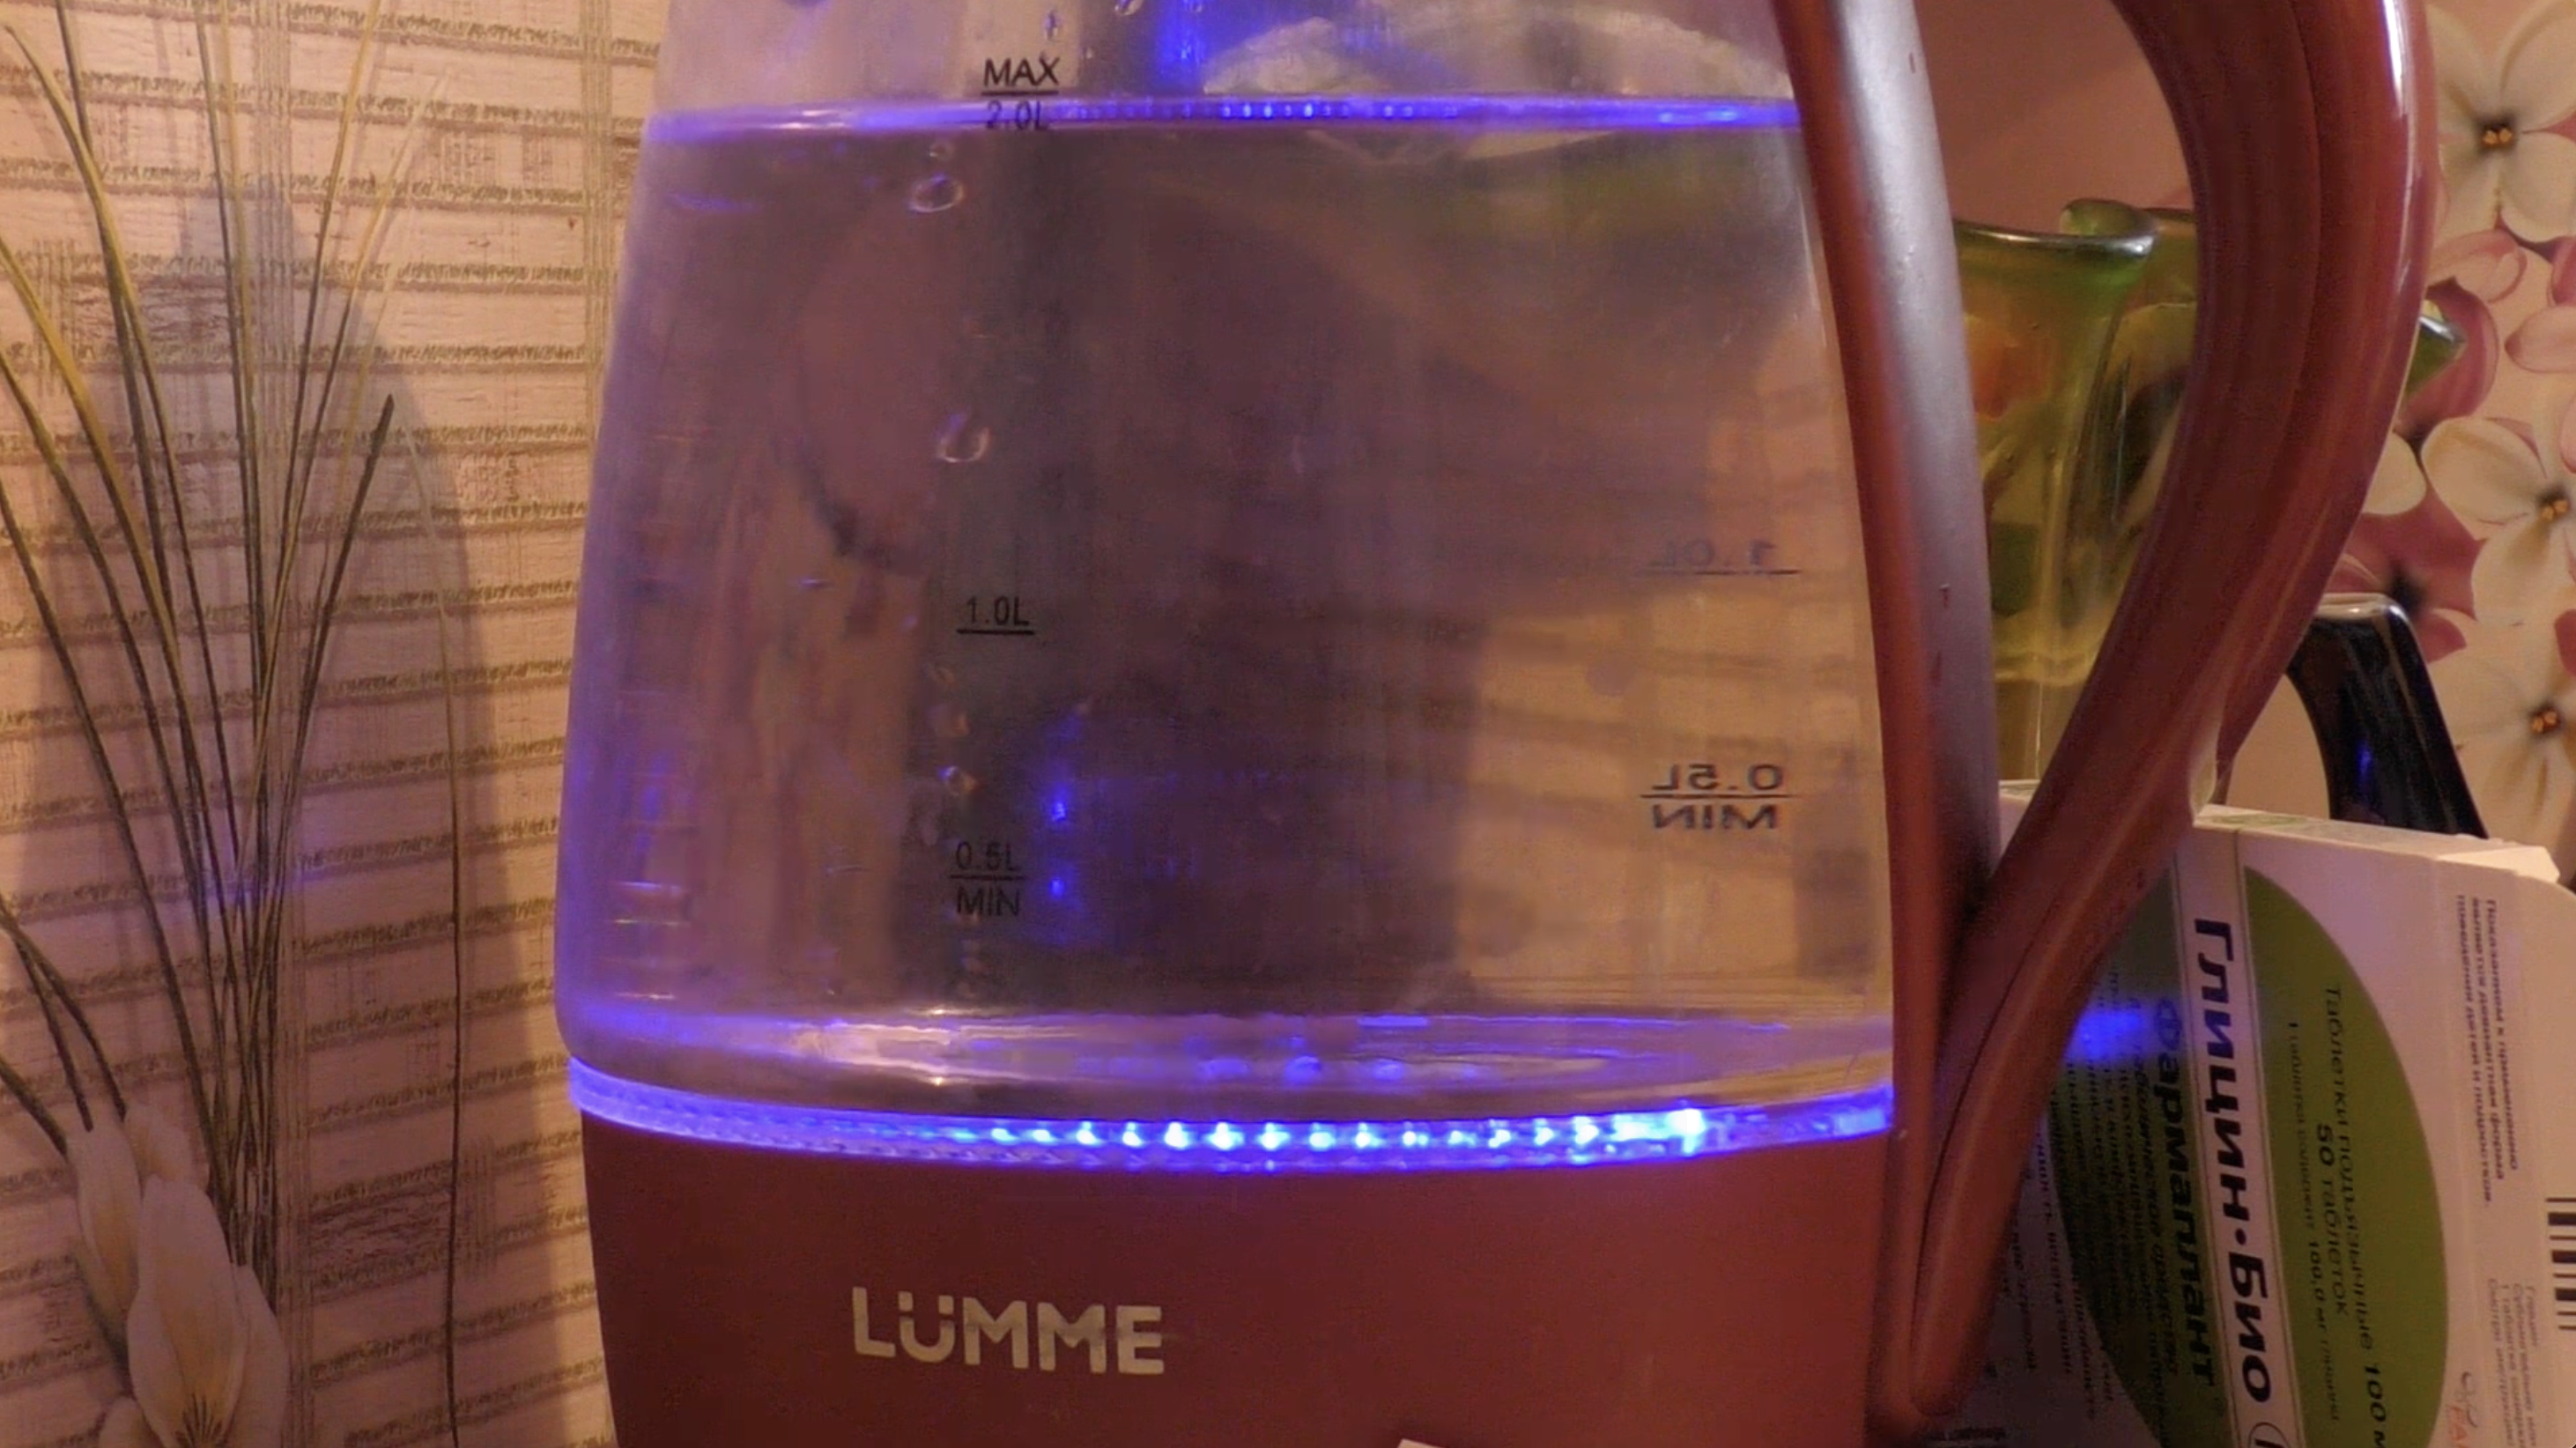
\includegraphics[width=0.7\textwidth]{images/image.png}
	\caption{Prasens + проверка.}
	\label{fig:syntdiag}
\end{figure}

%%%%%%%%%%%%%%%%%%%%%%%%%%%%%%%%%%%%%%%%%%%%%%%%%%%%%%%%%%%%%%%%%%%%%%%%
\newpage
\section*{Заключение}
\addcontentsline{toc}{section}{Заключение}

В данной работе была разработана и формально описана \textbf{LL(1)}‑грамматика для подмножества естественного языка - немецкого времени \textit{Plusquamperfekt}.  
Полученная грамматика является контекстно-свободной (КС), так как все правила имеют вид $A \to \alpha$, где $A \in N$ - нетерминал, а $\alpha \in (T \cup N)^*$ - цепочка из терминалов и нетерминалов. Наличие $\epsilon$-переходов в правилах вида $A \to \varepsilon$ также подтверждает принадлежность грамматики к классу КС-грамматик.

В коде на \textit{Haskell} реализованы:

\begin{itemize}
  \item генератор случайных предложений, строго подчинённых правилам грамматики;
  \item линейный распознаватель, проверяющий принадлежность строки языку.
\end{itemize}

\medskip
Кроме основной цели, модуль поддерживает ещё три подмножества естественных языков:

\begin{itemize}
  \item немецкое \textbf{Präsens} — согласование глаголов по лицу/числу;
  \item конструкцию \textbf{Modal + Infinitiv} (DE) с правильной формой модального глагола;
  \item азербайджанский \textbf{Present Perfect}‑шаблон «SUBJ ADV OBJ VERB», где глагол
        также согласуется с подлежащим.
\end{itemize}

Все реализованные грамматики являются контекстно-свободными, так как во всех реализован $\epsilon$-переход. Это означает, что порождаемые ими языки $L(G)$ также являются контекстно-свободными, где $G$ - соответствующая грамматика. Формально это можно записать как:

\[
L(G) = \{w \in T^* \mid S \Rightarrow^* w\}
\]

где $S$ - начальный символ грамматики, $T$ - множество терминалов, а $\Rightarrow^*$ - рефлексивно-транзитивное замыкание отношения вывода.

Грамматики также принадлежат классу $LL(1)$, что обеспечивает эффективный нисходящий разбор без возвратов.

%%%%%%%%%%%%%%%%%%%%%%%%%%%%%%%%%%%%%%%%%%%%%%%%%%%%%%%%%%%%%%%%%%%%%%%%%%%%%%% - CFG

\paragraph*{Плюсы реализации}
\begin{itemize}
  \item все четыре временные формы описаны одной архитектурой и содержат вспомогательные функции;
  \item грамматики действительно LL(1) — распознавание выполняется за $O(n)$;
  \item лексиконы вынесены в списки — легко дополнять словарь без изменения алгоритмов.
\end{itemize}

\paragraph*{Минусы}
\begin{itemize}
  \item не моделируется выбор \textit{sein/haben} в Plusquamperfekt;
  \item отсутствует род‑числовое согласование детерминатива и существительного;
  \item генерация пока не учитывает семантические ограничения (некоторые AUX–Partizip комбинации некорректны).
\end{itemize}

\paragraph*{Масштабирование}
\begin{itemize}
  \item добавить отрицательные и вопросительные формы (достаточно расширить правила и словари);
  \item учесть род и падеж с помощью системы признаков либо путём расширения лексиконов;
  \item внедрить таблицу выбора \textit{sein/haben} по классу глагола для более точного
        Plusquamperfekt;
  \item обобщить механизм согласования и использовать его для новых языков — модуль уже содержит примеры для немецкого и азербайджанского.
\end{itemize}

\newpage
%-------------------------  Приложение А  -------------------------------
\section*{Приложение А. Порождающая грамматика (Pluperfect)}
\addcontentsline{toc}{section}{Приложение А. Порождающая грамматика (Pluperfect)}
\begin{enumerate}
  \item $\langle S\rangle            ::= \langle NP_{\text{subj}}\rangle\;\langle VP_1\rangle$
  \item $\langle NP_{\text{subj}}\rangle ::= \langle Pronoun\rangle$
  \item $\langle VP_1\rangle         ::= \langle Aux\rangle\;\langle VP_2\rangle$
  \item $\langle Aux\rangle          ::= \text{auxsPlu}$
  \item $\langle VP_2\rangle         ::= \langle OptAdv\rangle\;\langle OptObj\rangle\;\langle V_{en}\rangle$
  \item $\langle OptAdv\rangle       ::= \langle Adv\rangle \;|\; \varepsilon$
  \item $\langle OptObj\rangle       ::= \langle NP_{\text{obj}}\rangle \;|\; \varepsilon$
  \item $\langle NP_{\text{obj}}\rangle ::= \langle Det\rangle\;\langle N\rangle$
  \item $\langle Det\rangle          ::= \text{determinersAcc}$
  \item $\langle N\rangle            ::= \text{nounsAcc}$
  \item $\langle Adv\rangle          ::= \text{adverbs}$
  \item $\langle V_{en}\rangle       ::= \text{pparts}$
  \item $\langle Pronoun\rangle      ::= \text{pronouns}$
\end{enumerate}
\end{document}